\onehalfspacing
\section{Đề số 18}
\graphicspath{{./img/}}
\begin{bt} 
    \hfil
    \begin{enumerate}[a.]
        \item So sánh: $\sqrt{17}+\sqrt{26}+1$ và $\sqrt{99}$.
        \item Chứng minh: $\frac{1}{\sqrt{1}}+\frac{1}{\sqrt{2}}+\frac{1}{\sqrt{3}}+\ldots .+\frac{1}{\sqrt{99}}+\frac{1}{\sqrt{100}}>10$.
        \item Cho $S=1-\frac{1}{2}+\frac{1}{3}-\frac{1}{4}+\ldots+\frac{1}{2013}-\frac{1}{2014}+\frac{1}{2015}$ và
        $$
        P=\frac{1}{1008}+\frac{1}{1009}+\frac{1}{1010}+\ldots+\frac{1}{2014}+\frac{1}{2015} \text {. }
        $$
        Tính $(S-P)^{2016}$.
    \end{enumerate}
\loigiai{
    \begin{enumerate}
        \item Ta có: $\sqrt{17}>\sqrt{16} ; \sqrt{26}>\sqrt{25}\\[5px] \Rightarrow \sqrt{17}+\sqrt{26}+1>\sqrt{16}+\sqrt{25}+1=4+5+1=10$\\[5px]
        Mà $10=\sqrt{100}>\sqrt{99}$\\[5px]
        Vậy: $\sqrt{17}+\sqrt{26}+1>\sqrt{99}$.\\[5px]
        \item Ta có: $\frac{1}{\sqrt{1}}>\frac{1}{\sqrt{100}} ; \frac{1}{\sqrt{2}}>\frac{1}{\sqrt{100}} ; \frac{1}{\sqrt{3}}>\frac{1}{\sqrt{100}} ; \ldots ; \frac{1}{\sqrt{99}}>\frac{1}{\sqrt{100}}$\\[5px]
        Suy ra: $\frac{1}{\sqrt{1}}+\frac{1}{\sqrt{2}}+\frac{1}{\sqrt{3}}+\ldots .+\frac{1}{\sqrt{100}}>100 \cdot \frac{1}{\sqrt{100}}=10$\\[5px]
        Vậy: $\frac{1}{\sqrt{1}}+\frac{1}{\sqrt{2}}+\frac{1}{\sqrt{3}}+\ldots+\frac{1}{\sqrt{100}}>10$
        \item$\text {Ta có: } P=\frac{1}{1008}+\frac{1}{1009}+\frac{1}{1010}+\ldots+\frac{1}{2014}+\frac{1}{2015} \\[5px]
            =\left(1+\frac{1}{2}+\frac{1}{3}+\ldots+\frac{1}{1006}+\frac{1}{1007}+\frac{1}{1008}+\ldots+\frac{1}{2014}+\frac{1}{2015}\right)-\left(1+\frac{1}{2}+\frac{1}{3}+\ldots+\frac{1}{1006}+\frac{1}{1007}\right) \\[5px]
            =\left(1+\frac{1}{2}+\frac{1}{3}+\ldots+\frac{1}{1006}+\frac{1}{1007}+\frac{1}{1008}+\ldots+\frac{1}{2014}+\frac{1}{2015}\right)-2\left(\frac{1}{2}+\frac{1}{4}+\frac{1}{6}+\ldots+\frac{1}{2012}+\frac{1}{2014}\right) \\[5px]
            =1-\frac{1}{2}+\frac{1}{3}-\frac{1}{4}+\ldots \ldots+\frac{1}{2013}-\frac{1}{2014}+\frac{1}{2015}=S . \\[5px]
            \text { Do đó }(S-P)^{2016}=0$
    \end{enumerate}
}
\end{bt}

\begin{bt}
    \hfill
	\begin{enumerate}[a.]
        \item Một số nguyên tố $\mathrm{p}$ chia cho 42 có số dư $\mathrm{r}$ là hợp số. Tìm hợp số $\mathrm{r}$.
        \item Tìm số tự nhiên $\overline{a b}$ sao cho $\overline{a b}^2=(a+b)^3$
    \end{enumerate}
	\loigiai{
        \begin{enumerate}
            \item Vì $\mathrm{p}$ chia cho 42 có số dư là $\mathrm{r}$ nên: $\mathrm{p}=42 \mathrm{k}+\mathrm{r}(0<\mathrm{r}<42, \mathrm{k}, \mathrm{r}$ tự nhiên)\\[5px]
            Hay $\mathrm{p}=2.3 .7 \mathrm{k}+\mathrm{r}$.\\[5px]
            Vì $\mathrm{p}$ là số nguyên tố nên $\mathrm{r}$ không chia hết cho $2 ; 3 ; 7$\\[5px]
            $\Rightarrow \mathrm{r}$ là hợp số không chia hết cho 2; $3 ; 7$ và $\mathrm{r}<42$\\[5px]
            Học sinh chỉ ra được $r=25$\\[5px]
            Vậy hợp số $r=25$\\[5px]
            \item Ta có: $(\mathrm{a}+\mathrm{b})^3=\overline{a b}^2$ là số chính phương nên $\mathrm{a}+\mathrm{b}$ là số chính phương.\\[5px]
            Đặt $\mathrm{a}+\mathrm{b}=\mathrm{x}^2\left(x \in N^*\right)$\\[5px]
            Suy ra: $\overline{a b}^2=(a+b)^3=\mathrm{x}^6$
            $\Rightarrow \mathrm{x}^3=\overline{a b}<100$ và $\overline{a b}>8 \Rightarrow 8<\mathrm{x}^3<100 \Rightarrow 2<\mathrm{x}<5 \Rightarrow \mathrm{x}=3 ; 4$ vì $\mathrm{x} \in N^*$\\[5px]
            - Nếu $x=3 \Rightarrow \overline{a b}^2=(a+b)^3=3^6=729=27^2=(2+7)^3 \Rightarrow \mathrm{x}=3$ (nhận)\\[5px]
            - Nếu x $=4 \Rightarrow \overline{a b}^2=(a+b)^3=4^6=4096=64^2 \neq(6+4)^3=1000$\\[5px]
            $\Rightarrow x=4$ (không thỏa mãn)\\[5px]
            Vậy số cần tìm là: $\overline{a b}=27$
        \end{enumerate}
    } 
\end{bt}

\begin{bt}
    \hfill
	\begin{enumerate}[a.]
        \item Cho $\mathrm{x} ; \mathrm{y} ; \mathrm{z} \neq 0$ và $\mathrm{x}-\mathrm{y}-\mathrm{z}=0$. Tính giá trị biểu thức $B=\left(1-\frac{z}{x}\right)\left(1-\frac{x}{y}\right)\left(1+\frac{y}{z}\right)$
        \item Cho $\frac{3 x-2 y}{4}=\frac{2 z-4 x}{3}=\frac{4 y-3 z}{2}$. Chứng minh rằng: $\frac{x}{2}=\frac{y}{3}=\frac{z}{4}$
         Cho biểu thức $M=\frac{5-x}{x-2}$. Tìm x nguyên để $\mathrm{M}$ có giá trị nhỏ nhất.
    \end{enumerate}
	\loigiai{
        \begin{enumerate}
            \item Ta có: $B=\left(1-\frac{z}{x}\right)\left(1-\frac{x}{y}\right)\left(1+\frac{y}{z}\right)=\frac{x-z}{x} \cdot \frac{y-x}{y} \cdot \frac{z+y}{z}$\\[5px]
            Từ: $\mathrm{x}-\mathrm{y}-\mathrm{z}=0 \Rightarrow \mathrm{x}-\mathrm{z}=\mathrm{y} ; \mathrm{y}-\mathrm{x}=-\mathrm{z}$ và $\mathrm{y}+\mathrm{z}=\mathrm{x}$\\[5px]   
            Suy ra: $\mathrm{B}=\frac{y}{x} \cdot \frac{-z}{y} \cdot \frac{x}{z}=-1(x ; y ; z \neq 0)$\\[5px]
            \item Ta có: $\frac{3 x-2 y}{4}=\frac{2 z-4 x}{3}=\frac{4 y-3 z}{2}\\[5px]=>\frac{4(3 x-2 y)}{16}=\frac{3(2 z-4 x)}{9}=\frac{2(4 y-3 z)}{4}$\\[5px]
            Áp dụng tính chất dãy tỉ số bằng nhau ta có:\\[5px]
            $\frac{4(3 x-2 y)}{16}=\frac{3(2 z-4 x)}{9}=\frac{2(4 y-3 z)}{4}=\frac{4(3 x-2 y)+3(2 z-4 x)+2(4 y-3 z)}{16+9+4}=0$\\[5px]
            $\Rightarrow\frac{4(3 x-2 y)}{16}=0\\[5px] \Rightarrow>3 x=2 y=>\frac{x}{2}=\frac{y}{3}(1) \text { và } \frac{3(2 z-4 x)}{9}=0\\[5px] \Rightarrow 2 z=4 x=>\frac{x}{2}=\frac{z}{4}(2)$\\[5px]
           Từ (1) và (2) suy ra: $\frac{x}{2}=\frac{y}{3}=\frac{z}{4}$
           \item Ta có: $M=\frac{5-x}{x-2}=\frac{3-(x-2)}{x-2}=\frac{3}{x-2}-1(x \neq 2)$\\[5px]
$M$ nhỏ nhất $\Leftrightarrow \frac{3}{x-2}$ nhỏ nhất $\Leftrightarrow x-2$ lớn nhất và $x-2<0$\\[5px]
$\Leftrightarrow x$ lớn nhât và $x<2 \Leftrightarrow x=1$ (vì $x$ nguyên)\\[5px]
Khi đó $G T N N$ của $M$ là: $M=\frac{3}{1-2}-1=-4$ khi $x=1$
        \end{enumerate}
    }
\end{bt}

\begin{bt}
   Cho $x A y=60^{\circ}$ vẽ tia phân giác $\mathrm{Az}$ của góc đó. Từ một điểm $\mathrm{B}$ trên tia $\mathrm{Ax}$ vẽ đường thẳng song song với $\mathrm{Ay}$ cắt $\mathrm{Az}$ tại $\mathrm{C}$. Kẻ $\mathrm{BH} \perp \mathrm{Ay}$ tại $\mathrm{H}, \mathrm{CM} \perp \mathrm{Ay}$ tại $\mathrm{M}, \mathrm{BK} \perp$ AC tại K. Chứng minh:
    \begin{enumerate}[a.]
        \item $\mathrm{KC}=\mathrm{KA}$
        \item $\mathrm{BH}=\frac{A C}{2}$
        \item $\triangle \mathrm{KMC}$ đều.
    \end{enumerate}
\loigiai{
    $$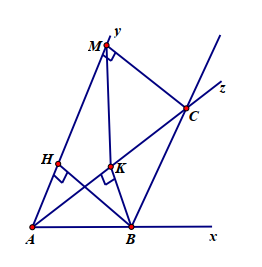
\includegraphics[width=0.4\textwidth]{18-4-lg.png}$$
    \begin{enumerate}
        \item Chứng minh: $\mathrm{KC}=\mathrm{KA}$\\[5px]
        Ta có $y A z=z A x=30^{\circ}(\mathrm{Az}$ là tia phân giác của $x A y$ )\\[5px]
        Mà: $y A z=A C B(\mathrm{Ay} / / \mathrm{BC}$, so le trong)\\[5px]
        $\Rightarrow \approx A x=A C B \Rightarrow \triangle A B C$ cân tại $\mathrm{B}$\\[5px]
        Trong tam giác cân $\mathrm{ABC}$ có $\mathrm{BK}$ là đường cao ứng với cạnh đáy\\[5px]
        $\Rightarrow \mathrm{BK}$ cũng là đường trung tuyến của $\triangle \mathrm{ABC} \Rightarrow \mathrm{KC}=\mathrm{KA}$\\[5px]
        \item Chứng minh: $\mathrm{BH}=\frac{A C}{2}$\\[5px]
        Ta có: $A B H=90^{\circ}-x A y=30^{\circ}(\triangle \mathrm{ABH}$ vuông tại $\mathrm{H})$.\\[5px]
        Xét hai tam giác vuông $\triangle \mathrm{ABH}$ và $\triangle \mathrm{BAK}$, có:\\[5px]
        $\mathrm{AB}$ : Cạnh chung; $=A x=A B H\left(=30^{\circ}\right)$\\[5px]
        $\Rightarrow \triangle \mathrm{ABH}=\Delta \mathrm{BAK} \Rightarrow \mathrm{BH}=\mathrm{AK}$\\[5px]
        Mà: $\mathrm{AK}=\frac{A C}{2}(c m t) \Rightarrow B H=\frac{A C}{2}$\\[5px]
        \item Chứng minh: $\triangle \mathrm{KMC}$ đều\\[5px]
        Ta có: $\triangle \mathrm{AMC}$ vuông tại $\mathrm{M}$ có $\mathrm{MK}$ là trung tuyến ứng với cạnh huyền \\[5px]$\Rightarrow \mathrm{KM}=\mathrm{AC} / 2$\\[5px]
        Mà: $\mathrm{AK}=\mathrm{KC}=\mathrm{AC} / 2(2)$\\[5px]
        Từ (1) và (2) $=>\mathrm{KM}=\mathrm{KC} \Rightarrow \Delta \mathrm{KMC}$ cân tại $\mathrm{K}$ (3)\\[5px]
        Mặt khác: $\triangle \mathrm{AMC}$ có $A M C=90^{\circ} ; \mathrm{yAz}=30^{\circ} \Rightarrow M C K=90^{\circ}-30^{\circ}=60^{\circ}$\\[5px]
        Từ (3) và (4) $\Rightarrow \triangle \mathrm{AMC}$ đều
    \end{enumerate}
}
\end{bt}

\begin{bt}
   Cho $\Delta \mathrm{ABC}$ có $B=2 \cdot C<90^{\circ}$. Vẽ $\mathrm{AH}$ vuông góc với $\mathrm{BC}$ tại $\mathrm{H}$. Trên tia $\mathrm{AB}$ lấy điểm $\mathrm{D}$ sao cho $\mathrm{AD}=\mathrm{HC}$. Chứng minh rằng đường thẳng $\mathrm{DH}$ đi qua trung điểm của đoạn thẳng $\mathrm{AC}$.
\loigiai{
    $$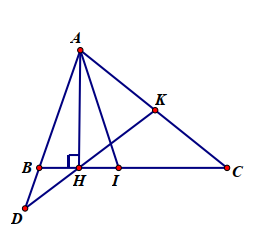
\includegraphics[width=0.4\textwidth]{18-5-lg.png}$$
    Ta có: $B=2 . C \Rightarrow B>C$ nên $\mathrm{AC}>\mathrm{AB} \Rightarrow \mathrm{HC}>\mathrm{HB}$\\[5px]
Trên đoạn thẳng $\mathrm{HC}$ lấy điểm $\mathrm{I}$ sao cho $\mathrm{IH}=\mathrm{HB} \Rightarrow \Delta \mathrm{AHI}$ $=\Delta \mathrm{AHB}$\\[5px]
$\Rightarrow \mathrm{AI}=\mathrm{AB}$ và $A I B=A B C=2 \cdot A C B$\\[5px]
Mặt khác: $A I B=A C B+I A C \Rightarrow I A C=A C B$\\[5px]
Do đó: $\mathrm{IA}=\mathrm{IC}<\mathrm{HC}$ hay $\mathrm{AB}<\mathrm{HC}=\mathrm{AD}$\\[5px]
Gọi $\mathrm{K}$ là giao điểm của $\mathrm{DH}$ với $\mathrm{AC}$.\\[5px]
Vì $\mathrm{AD}=\mathrm{HC}, \mathrm{AB}=\mathrm{IC}$ nên $\mathrm{BD}=\mathrm{HI}=\mathrm{HB} \Rightarrow \Delta \mathrm{DBH}$ cân tại $\mathrm{B}$\\[5px]
Do đó: $B D H=B H D=\frac{1}{2} A B C=A C B$\\[5px]
Suy ra: $K H C=A C B(=B H D) \Rightarrow K A H=K H A$ (phụ hai góc bằng nhau)\\[5px]
Suy ra: $\mathrm{KA}=\mathrm{KH}=\mathrm{KC}$ hay $\mathrm{K}$ là trung điểm của $\mathrm{AC}$\\[5px]
Vậy đường thẳng $\mathrm{DH}$ đi qua trung điểm của đoạn thẳng $\mathrm{AC}$
}
\end{bt}

